\documentclass[conference]{IEEEtran}
\IEEEoverridecommandlockouts
\usepackage{amsmath,amssymb,amsfonts}
\usepackage{algorithm}
\usepackage{algorithmic}
\usepackage{graphicx}
\graphicspath{{images/}}
\usepackage{textcomp}
\usepackage{xcolor}
\usepackage{booktabs}
\usepackage{array}
\usepackage{url}
\usepackage{cite}
\usepackage[compact]{titlesec}
\titlespacing{\section}{0pt}{4pt plus 1pt minus 1pt}{2pt plus 1pt minus 1pt}
\titlespacing{\subsection}{0pt}{3pt plus 1pt minus 1pt}{1.5pt plus 1pt minus 1pt}
\usepackage{tikz}
\usetikzlibrary{arrows.meta,positioning,shapes.geometric}

\setlength{\floatsep}{3pt plus 1pt minus 1pt}
\setlength{\dblfloatsep}{3pt plus 1pt minus 1pt}
\setlength{\textfloatsep}{3pt plus 1pt minus 1pt}
\setlength{\dbltextfloatsep}{3pt plus 1pt minus 1pt}
\setlength{\intextsep}{3pt plus 1pt minus 1pt}
\setlength{\abovecaptionskip}{1.5pt plus 0.5pt minus 0.5pt}
\setlength{\belowcaptionskip}{1.5pt plus 0.5pt minus 0.5pt}
\setlength{\abovedisplayskip}{3pt plus 1pt minus 2pt}
\setlength{\belowdisplayskip}{3pt plus 1pt minus 2pt}
\setlength{\abovedisplayshortskip}{2pt plus 1pt}
\setlength{\belowdisplayshortskip}{2pt plus 1pt}

\def\BibTeX{{\rm B\kern-.05em{\sc i\kern-.025em b}\kern-.08em
    T\kern-.1667em\lower.7ex\hbox{E}\kern-.125emX}}

\begin{document}

\title{
\textbf{Application of TCN and Transformer Networks for Log Anomaly Detection in Large-Scale Enterprise and Industrial Networks}\\[0.8em]
}

\author{\IEEEauthorblockN{Hoang-Tu Trinh\thanks{The complete source code, configuration files, and instructions for obtaining and preprocessing the public HDFS and BGL datasets are available at: \protect\url{https://github.com/thtcsec/vnict2026-log-anomaly}.}}
\IEEEauthorblockA{\textit{Department of Information Technology} \\
\textit{Ho Chi Minh City University of} \\
\textit{Foreign Languages - Information Technology} \\
\textit{(HUFLIT)}\\
Ho Chi Minh City, Vietnam \\
Email: tht.csec2005@gmail.com}
\and
\IEEEauthorblockN{Tien-Thanh Cao}
\IEEEauthorblockA{\textit{Department of Information Technology} \\
\textit{Ho Chi Minh City University of} \\
\textit{Foreign Languages - Information Technology} \\
\textit{(HUFLIT)}\\
Ho Chi Minh City, Vietnam \\
Email: thanhct@huflit.edu.vn}
}

\maketitle

\begin{abstract}
This paper presents a large-scale system log anomaly detection pipeline based on Drain3 and event sequence analysis, comparing Temporal Convolutional Networks (TCN) and Transformers against traditional baselines on two large-scale system log datasets. Raw logs are parsed into event templates, grouped into sequences, and scored for anomalies using five branches: PCA/SVD, Isolation Forest, DeepLog (LSTM next-event prediction), TCN (Temporal Convolutional Network), and Transformer masked event modeling. On HDFS (500k lines, 137 templates), experiments across five random seeds show that PCA achieves an F1-score of $0.5711 \pm 0.0944$, slightly outperforming DeepLog and TCN ($0.4613 \pm 0.0199$). On BGL (500k lines, 198 templates, window size $W=100$), TCN achieves the highest mean F1-score of $0.9826 \pm 0.0022$ in top-$k$ mode, although its margin over DeepLog LSTM ($0.9820 \pm 0.0042$) is small relative to seed variation. In NLL mode, TCN reaches $0.9474 \pm 0.0035$, compared with $0.9381 \pm 0.0075$ for DeepLog and $0.9388 \pm 0.0080$ for the validation-tuned Transformer. Under the tested configuration, TCN demonstrates a competitive classification profile on BGL and efficient inference latency compared to LSTM and Transformer models, while PCA remains competitive on short-sequence datasets such as HDFS. The contributions include: (i) a reproducible evaluation pipeline with strict leakage prevention; (ii) a multi-dataset comparative evaluation on HDFS and BGL; (iii) a grouping strategy study on fixed and sliding windows; (iv) ablation studies on Drain3 threshold, top-$k$, and mask ratio; and (v) inference-latency and qualitative explainability analyses.
\end{abstract}

\begin{IEEEkeywords}
Log anomaly detection, masked event modeling, Transformer, Drain3, AIOps, distributed systems.
\end{IEEEkeywords}

\section{Introduction}
Modern large-scale computing infrastructures, including distributed storage systems, supercomputers, web services, and cloud platforms, generate logs with diverse formats and frequencies. These system logs capture both the operational state and the behavioral patterns of running services, while manually crafted detection rules quickly become obsolete as the infrastructure evolves. Effective log anomaly detection therefore requires analysis at the event sequence level rather than individual log lines.

This paper is positioned as an applied research and system evaluation study, rather than proposing a new anomaly detection algorithm. The central idea is to treat the event template sequence after Drain3 parsing as an intermediate representation layer: compact enough to run lightweight baselines, structured enough to extend to sequence models, and clear enough to map to operational units such as sessions, anonymized users, or time windows. Three research questions are addressed:
\begin{itemize}
    \item \textbf{RQ1:} How does the method of constructing event sequences after Drain3 affect the anomaly detection signal?
    \item \textbf{RQ2:} How do the five scoring branches (reconstruction, isolation, next-event prediction, causal convolution, and masked event modeling) compare on the same event sequence?
    \item \textbf{RQ3:} Does the performance ranking of these branches remain consistent when moving from HDFS to BGL (datasets with very different characteristics)?
\end{itemize}

The main contributions include: (1) an end-to-end pipeline of Drain3 parsing, event sequencing, and anomaly scoring with five alternative branches (PCA/SVD, Isolation Forest, DeepLog, TCN, and Transformer masked event modeling); (2) a multi-seed evaluation (five random seeds) on HDFS with a protocol that prevents test set leakage, along with a grouping strategy study for Block ID, fixed window, and sliding window; (3) a multi-dataset comparative evaluation on HDFS and BGL on the same pipeline; (4) an ablation study for Drain3 threshold, DeepLog top-$k$, and Transformer mask ratio; (5) an inference latency benchmark, Error Taxonomy and Analysis, and qualitative explainability case study for deployment-oriented interpretation.

\section{Related Work}
The earliest log anomaly detection methods typically represented log data as event count vectors or feature matrices, and then applied traditional machine learning models such as PCA, clustering, or Isolation Forest \cite{b10,b11}. PCA is used to separate normal behavior space and detect points deviating from the principal subspace. This group of methods is lightweight and easy to deploy, but usually ignores the temporal order and contextual relationships between log events.

To address this limitation, sequential models like DeepLog \cite{b1} use LSTM networks to predict the next event based on previous events. LogAnomaly \cite{b13} and LogRobust \cite{b14} extend this direction by combining sequential and semantic log information to deal with unstable log data. Additionally, semi-supervised approaches such as PLELog \cite{b15} use probabilistic label estimation to reduce dependence on manual labels. Overall, RNN/LSTM architectures capture sequence relationships better than traditional statistical methods, but still suffer from sequential processing limitations and are difficult to parallelize.

To represent unstructured logs for machine learning models, log parsing techniques are used to map each log line to a template. Drain \cite{b3} and Drain3 are widely used due to their fixed-depth parse tree structure, which allows high-speed online parsing. Recently, LogPPT \cite{b7} used prompt-based few-shot learning to improve parsing accuracy when labeled data is scarce.

The Transformer architecture with its self-attention mechanism \cite{b4} has been widely applied in AIOps. LogBERT \cite{b2} employs a Transformer encoder combined with masked event modeling to learn bidirectional representations for normal log sequences, improving contextual anomaly detection. Survey papers also note a strong shift from traditional sequential models to self-supervised deep learning based on Transformers \cite{b16}. In parallel, Large Language Model (LLM) and prompt learning approaches such as LogPrompt \cite{b8} and LogGPT \cite{b9} enhance semantic understanding, but face major barriers in terms of inference cost and real-time latency.

\begin{table}[htbp]
\caption{Comparison of methodology groups and research gaps}
\begin{center}
\scriptsize
\setlength{\tabcolsep}{3pt}
\begin{tabular}{lp{1.6cm}p{2.3cm}p{2.1cm}}
\toprule
\textbf{Group} & \textbf{Representatives} & \textbf{Key Limitation} & \textbf{Improvement in This Work} \\
\midrule
Statistical & PCA, IF \cite{b10,b11} & No temporal ordering & Lightweight baseline quantification \\
Sequential & DeepLog \cite{b1,b13} & Limited sequence length, sequential bottleneck & Parallel TCN integration \\
Transformer & LogBERT \cite{b2} & Dependent on parsing quality & Decoupled parsing, grouping, and scoring \\
\bottomrule
\end{tabular}
\label{tab_related_work}
\end{center}
\end{table}

From existing works, four main research gaps can be identified: (i) traditional statistical methods do not learn the order of log events; (ii) sequential LSTM models are limited with long log sequences; (iii) Transformer models depend heavily on the parsing step; (iv) mapping anomaly detection pipelines to large networks requires clarifying the grouping strategy and business scenarios. 

To address these gaps, this paper builds a standardized pipeline that separates three phases (parsing, grouping, and scoring) using Drain3 as a preprocessing step to clean the token space. We evaluate in parallel the scoring branches including lightweight baselines (PCA, TruncatedSVD, Isolation Forest), sequential LSTM (DeepLog), the integrated Temporal Convolutional Network (TCN), and Transformer masked event modeling. Performance is carefully measured using Precision, Recall, and F1-score averaged over five different random seeds to ensure scientific reliability. The complete source code, configuration files, and instructions for obtaining and preprocessing the public HDFS and BGL datasets are available at \url{https://github.com/thtcsec/vnict2026-log-anomaly}.

\section{Proposed Methodology}
\subsection{Pipeline Overview}
The proposed pipeline is designed to clearly separate three processing layers: log standardization, event sequence construction, and anomaly detection. The input is a raw log dataset $L=\{l_1,l_2,\ldots,l_N\}$ generated from the operating system. The output is an anomaly label or score $a(S)$ for each event sequence $S$. In HDFS experiments, a sequence corresponds to a Block ID; in BGL experiments, a sequence corresponds to a fixed-size time window. In broader deployment scenarios, a sequence can correspond to a login session, an anonymized user, a service, or a sliding time window.

\begin{figure}[!t]
\centering
\resizebox{0.83\columnwidth}{!}{
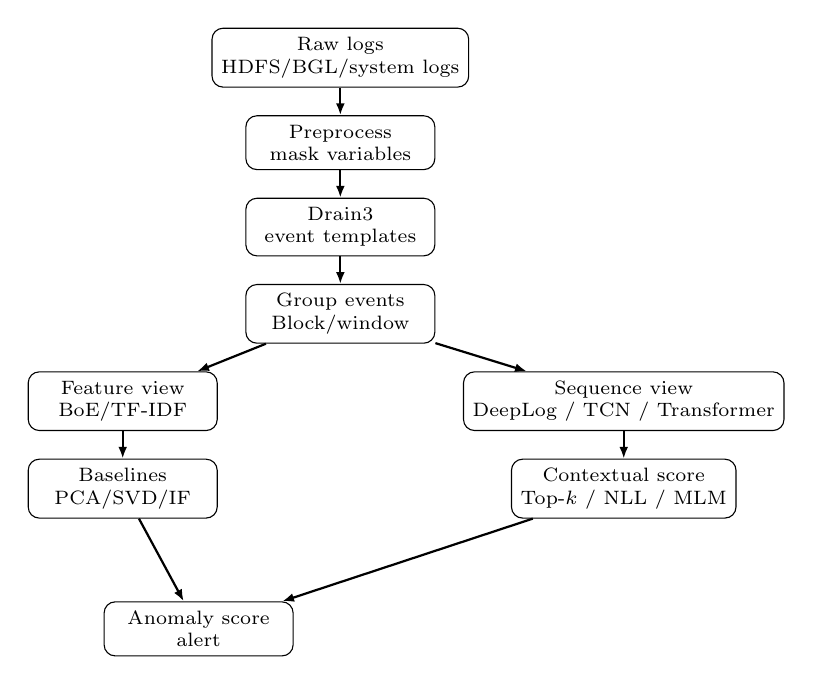
\begin{tikzpicture}[
    node distance=0.35cm and 0.35cm,
    box/.style={rectangle, draw, rounded corners, align=center, minimum width=2.4cm, minimum height=0.5cm, font=\scriptsize},
    arrow/.style={-{Latex[length=1.5mm]}, thick}
]
\node[box] (raw) {Raw logs\\HDFS/BGL/system logs};
\node[box, below=of raw] (pre) {Preprocess\\mask variables};
\node[box, below=of pre] (parse) {Drain3\\event templates};
\node[box, below=of parse] (seq) {Group events\\Block/window};
\node[box, below left=of seq] (vec) {Feature view\\BoE/TF-IDF};
\node[box, below=of vec] (base) {Baselines\\PCA/SVD/IF};
\node[box, below right=of seq] (bert) {Sequence view\\DeepLog / TCN / Transformer};
\node[box, below=of bert] (seqscore) {Contextual score\\Top-$k$ / NLL / MLM};
\node[box, below right=1.05cm and -1.45cm of base] (score) {Anomaly score\\alert};
\draw[arrow] (raw) -- (pre);
\draw[arrow] (pre) -- (parse);
\draw[arrow] (parse) -- (seq);
\draw[arrow] (seq) -- (vec);
\draw[arrow] (vec) -- (base);
\draw[arrow] (seq) -- (bert);
\draw[arrow] (bert) -- (seqscore);
\draw[arrow] (base) -- (score);
\draw[arrow] (seqscore) -- (score);
\end{tikzpicture}
}
\caption{Proposed log anomaly detection pipeline block diagram}
\label{fig_pipeline}
\end{figure}

The overall process consists of six steps:
\begin{itemize}
    \item \textbf{Step 1 -- Log Collection:} receive logs from source systems such as HDFS, BGL, or other structured system log sources.
    \item \textbf{Step 2 -- Preprocessing:} normalize variable fields such as timestamps, IPs, user IDs, session IDs, and query parameters.
    \item \textbf{Step 3 -- Log Parsing:} use Drain3 to map each log line to an event template and event ID.
    \item \textbf{Step 4 -- Event Grouping:} group event IDs by Block ID or by session/time window to create event sequences.
    \item \textbf{Step 5 -- Feature Representation:} generate bag-of-events/TF-IDF representation for baselines or keep the raw event sequence for sequence models.
    \item \textbf{Step 6 -- Anomaly Detection:} compute anomaly scores using reconstruction error, Isolation Forest, or sequence learning models.
\end{itemize}

Beyond the HDFS and BGL benchmarks evaluated in this study, the pipeline architecture is designed to accommodate other structured log sources after appropriate preprocessing and anonymization.

\subsection{Preprocessing, Drain3 Parsing, and Event Grouping}
The input is a raw log set $L=\{l_1,l_2,\ldots,l_N\}$. The process consists of: (i) normalizing variable parameters (IP, timestamp, ID); (ii) parsing raw logs into event templates using Drain3 \cite{b3}; (iii) grouping event IDs into sequences by Block ID or time windows.

Drain3 uses a fixed-depth tree to find the corresponding event template for each log line. The similarity between two log lines $T_1, T_2$ is calculated as the ratio of matching tokens:
\begin{equation}
Sim(T_1, T_2) = \frac{1}{n} \sum_{i=1}^{n} equ(t_{1,i}, t_{2,i})
\label{eq_sim}
\end{equation}
If $Sim(T_1, T_2) > st$ (similarity threshold, default 0.5), the log line is assigned to an existing template; otherwise, Drain3 creates a new template. After this step, each template is assigned an event ID, and the log sequence is represented as $S = [E_1, E_2, ..., E_m]$.
For HDFS, the sequence $S$ is grouped by Block ID. For BGL, it is grouped by non-overlapping windows of $W{=}100$ lines.

\subsection{Lightweight Machine Learning Baselines}
PCA and TruncatedSVD are applied to the bag-of-events vector representation $x = [count(E_j, S)]_{j=1}^d$ to learn the normal behavior subspace. The anomaly score is computed as the reconstruction error:
\begin{equation}
score(S)=\frac{1}{d}\sum_{j=1}^{d}(x_j-\hat{x}_j)^2
\label{eq_reconstruction}
\end{equation}
where $\hat{x}$ is the reconstructed vector after projecting onto the low-dimensional space (20 principal components by default). The threshold $\tau$ is chosen as the 95th percentile on normal training scores. Isolation Forest is applied to TF-IDF feature representations.

\subsection{Deep Sequence Models and Transformer}
\textbf{DeepLog (LSTM):} Replicated as next-event prediction using a 2-layer LSTM \cite{b1}. For position $i$, it predicts $E_i$ given context window $g{=}10$:
\begin{equation}
\hat{P}(E_i \mid E_{i-g}, \ldots, E_{i-1}) = \text{softmax}(W_o h_i + b_o)
\end{equation}
In top-$k$ mode ($K{=}9$), an alert triggers if an event lies outside the top $K$ predictions. In NLL mode, score is mean negative log-likelihood.

\textbf{Temporal Convolutional Network (TCN):} Integrated to improve parallelization and expand the receptive field using dilated causal 1D convolutions \cite{b19}:
\begin{equation}
F(s) = (x *_d f)(s) = \sum_{j=0}^{k-1} f(j) \cdot x_{s - d \cdot j}
\end{equation}
A Chomp1d mechanism crops padding to ensure causality.

\textbf{Transformer (LogBERT-inspired):} Employs a Transformer Encoder with masked event modeling \cite{b2}. A proportion of events ($r{=}0.15$) are replaced by \texttt{[MASK]} tokens, recovered via cross-entropy loss:
\begin{equation}
L_{MLM} = -\sum_{i \in M} \log P(k_i \mid S_{masked})
\label{eq_loss}
\end{equation}
The score is averaged over masked positions. Anomaly decisions apply threshold $\tau$ selected at the 95th percentile on the validation set.

% Position large 2-column tables early in TeX so LaTeX places them naturally on Pages 3 and 4
\begin{table*}[!t]
\caption{Multi-dataset performance comparison, reported as mean $\pm$ standard deviation over five random seeds.}
\centering
\scriptsize
\setlength{\tabcolsep}{3pt}
\begin{tabular}{l ccc ccc}
\toprule
& \multicolumn{3}{c}{\textbf{HDFS}} & \multicolumn{3}{c}{\textbf{BGL}} \\
\cmidrule(lr){2-4} \cmidrule(lr){5-7}
\textbf{Method} & \textbf{Precision} & \textbf{Recall} & \textbf{F1} & \textbf{Precision} & \textbf{Recall} & \textbf{F1} \\
\midrule
PCA & $0.6274 \pm 0.1944$ & $0.5450 \pm 0.0055$ & $0.5711 \pm 0.0944$ & $0.9473 \pm 0.0113$ & $0.8976 \pm 0.0144$ & $0.9217 \pm 0.0098$ \\
TruncatedSVD & $0.4298 \pm 0.2555$ & $0.5527 \pm 0.0106$ & $0.4540 \pm 0.1366$ & $0.9462 \pm 0.0051$ & $0.9255 \pm 0.0228$ & $0.9356 \pm 0.0117$ \\
Isolation Forest & $0.1726 \pm 0.0146$ & $0.1080 \pm 0.0084$ & $0.1328 \pm 0.0103$ & $0.1110 \pm 0.0171$ & $0.0248 \pm 0.0045$ & $0.0404 \pm 0.0070$ \\
\midrule
Transformer (unsup.) & $0.2094 \pm 0.0490$ & $0.2982 \pm 0.0892$ & $0.2458 \pm 0.0639$ & $0.9422 \pm 0.0110$ & $0.9073 \pm 0.0216$ & $0.9242 \pm 0.0085$ \\
Transformer (val-tuned) & $0.5102 \pm 0.1497$ & $0.2365 \pm 0.1156$ & $0.2950 \pm 0.0693$ & $0.9841 \pm 0.0017$ & $0.8975 \pm 0.0157$ & $0.9388 \pm 0.0080$ \\
DeepLog (top-$k$)* & $0.9862 \pm 0.0201$ & $0.3013 \pm 0.0167$ & $0.4613 \pm 0.0199$ & $0.9654 \pm 0.0083$ & $\mathbf{0.9991 \pm 0.0012}$ & $0.9820 \pm 0.0042$ \\
DeepLog (NLL) & $0.2644 \pm 0.0198$ & $0.3601 \pm 0.0256$ & $0.3046 \pm 0.0198$ & $0.9408 \pm 0.0066$ & $0.9355 \pm 0.0157$ & $0.9381 \pm 0.0075$ \\
\midrule
\textbf{TCN (top-$k$)}* & $0.9862 \pm 0.0201$ & $0.3013 \pm 0.0167$ & $0.4613 \pm 0.0199$ & $\mathbf{0.9666 \pm 0.0039}$ & $\mathbf{0.9991 \pm 0.0012}$ & $\mathbf{0.9826 \pm 0.0022}$ \\
\textbf{TCN (NLL)} & $0.2621 \pm 0.0277$ & $0.3644 \pm 0.0291$ & $0.3042 \pm 0.0236$ & $0.9412 \pm 0.0085$ & $0.9537 \pm 0.0094$ & $\mathbf{0.9474 \pm 0.0035}$ \\
\bottomrule
\multicolumn{7}{l}{\scriptsize *Note: Although DeepLog and TCN have different architectures, their top-$k$ decisions on HDFS are identical under the tested configuration.}\\
\multicolumn{7}{l}{\scriptsize One plausible explanation is short sequence length and small event vocabulary, limiting top-$k$ membership variation. Models produce different NLL scores.}
\end{tabular}
\label{tab_cross_dataset}
\end{table*}

\begin{table*}[!t]
\begin{minipage}[t]{0.48\textwidth}
\centering
\caption{Hyperparameter ablation study on HDFS 200k (seed 42)}
\label{tab_ablation}
\scriptsize
\setlength{\tabcolsep}{3pt}
\begin{tabular}{lcccc}
\toprule
\textbf{Configuration} & \textbf{Templates} & \textbf{Precision} & \textbf{Recall} & \textbf{F1} \\
\midrule
\multicolumn{5}{l}{\textit{(A) Drain3 $\theta$, evaluated on PCA reconstruction}} \\
$\theta=0.3$ & 25 & 0.3695 & 0.5215 & 0.4325 \\
$\theta=0.5$ \textbf{(default)} & 68 & 0.4070 & 0.5550 & \textbf{0.4696} \\
$\theta=0.7$ & 2455 & 0.1000 & 0.0287 & 0.0446 \\
\midrule
\multicolumn{5}{l}{\textit{(B) DeepLog top-$k$}} \\
$K=1$ & 68 & 0.0466 & 0.6403 & 0.0869 \\
$K=3$ & 68 & 0.9091 & 0.2878 & 0.4372 \\
$K=5$ & 68 & 0.9524 & 0.2878 & 0.4420 \\
$K=9$ \textbf{(default)} & 68 & 0.9756 & 0.2878 & \textbf{0.4444} \\
$K=15$ & 68 & 0.9750 & 0.2806 & 0.4358 \\
\midrule
\multicolumn{5}{l}{\textit{(C) Transformer mask ratio $r$}} \\
$r=0.10$ & 68 & 0.1615 & 0.2230 & 0.1873 \\
$r=0.15$ \textbf{(default)} & 68 & 0.1968 & 0.2662 & \textbf{0.2263} \\
$r=0.20$ & 68 & 0.1711 & 0.2302 & 0.1963 \\
$r=0.30$ & 68 & 0.1701 & 0.2374 & 0.1982 \\
\bottomrule
\end{tabular}
\end{minipage}
\hfill
\begin{minipage}[t]{0.48\textwidth}
\centering
\caption{Per-sample inference latency, batch size 1, averaged over 1,000 HDFS samples (unit: ms)}
\label{tab_latency}
\scriptsize
\setlength{\tabcolsep}{3pt}
\begin{tabular}{lcccc}
\toprule
\textbf{Branch} & \textbf{Mean} & \textbf{p95} & \textbf{p99} & \textbf{Throughput} \\
\midrule
Drain3 parse 1 line & 0.007 & 0.010 & 0.023 & 147,458 logs/s \\
PCA reconstruction & 0.063 & 0.153 & 0.219 & 15,869 sequences/s \\
TruncatedSVD & 0.176 & 0.281 & 0.381 & 5,689 sequences/s \\
Isolation Forest & 4.944 & 9.015 & 11.396 & 202 sequences/s \\
DeepLog (CPU) & 1.743 & 2.086 & 2.407 & 574 sequences/s \\
DeepLog (GPU) & 0.489 & 0.798 & 0.962 & 2,046 sequences/s \\
\textbf{TCN (CPU)} & 1.648 & 2.096 & 2.609 & 607 sequences/s \\
\textbf{TCN (GPU)} & 0.455 & 0.780 & 0.950 & 2,198 sequences/s \\
Transformer (CPU) & 2.395 & 2.966 & 3.267 & 418 sequences/s \\
Transformer (GPU) & 2.916 & 4.323 & 4.889 & 343 sequences/s \\
\bottomrule
\end{tabular}
\end{minipage}
\end{table*}

\section{Experimental Setup}
\subsection{Datasets}
The study uses HDFS and BGL from the LogHub benchmark \cite{b6,b12}. For computationally controlled evaluation, we use the first 500,000 log lines from each dataset while preserving their original chronological order. No random line-level sampling is performed before event grouping. This choice enables identical data-volume settings across datasets and reproducible experiments under limited computational resources. However, using the earliest segment may underrepresent later operational regimes and concept drift; therefore, the reported results should not be interpreted as estimates over the complete datasets.

Table~\ref{tab_dataset_stats} summarizes post-parsing statistics. Table~\ref{tab_dataset_comparison} outlines the structural properties contrasting HDFS and BGL.

\begin{table}[!t]
\caption{Statistics of HDFS and BGL datasets used in the experiments}
\begin{center}
\scriptsize
\begin{tabular}{lcc}
\toprule
\textbf{Metric} & \textbf{HDFS} & \textbf{BGL} \\
\midrule
Raw log lines & 500,000 & 500,000 \\
Grouping unit & Block ID & Window ($W{=}100$) \\
Number of sequences/windows & 36,305 & 5,000 \\
Number of normal sequences & 34,558 & 2,657 \\
Number of anomalous sequences & 1,747 & 2,343 (47\%) \\
Number of event templates (Drain3) & 137 & 198 \\
Drain3 similarity threshold $\theta$ & 0.5 & 0.5 \\
Drain3 tree depth & 4 & 4 \\
\bottomrule
\end{tabular}
\label{tab_dataset_stats}
\end{center}
\end{table}

\begin{table}[!t]
\caption{Structural differences between HDFS and BGL benchmarks}
\begin{center}
\scriptsize
\setlength{\tabcolsep}{2pt}
\begin{tabular}{lll}
\toprule
\textbf{Property} & \textbf{HDFS} & \textbf{BGL} \\
\midrule
Grouping unit & Block ID & Fixed line window ($W{=}100$) \\
Mean sequence length & 13.77 events & 100 events / window \\
Anomaly ratio & 4.8\% (Highly imbalanced) & 47.0\% (Near-balanced) \\
Label granularity & Block-level label & Window contains alert log \\
Event templates & 137 templates & 198 templates \\
Observed discriminative pattern & Event frequency shift & Temporal state transition \\
\bottomrule
\end{tabular}
\label{tab_dataset_comparison}
\end{center}
\end{table}

\textbf{Execution Environment:} Experiments were deployed on an Intel Core i7-13620H CPU, RTX 4050 6GB GPU, 16GB RAM, Ubuntu 22.04, Python 3.9, and PyTorch 2.0.

\textbf{Experimental Procedure and Parameters:} Data are split into train/test sets with a 70/30 ratio (baselines) or train/val/test with a 60/20/20 ratio (Transformer). The Transformer requires a dedicated validation partition for threshold calibration, whereas the remaining branches select thresholds exclusively from normal training scores. Therefore, comparisons involving the Transformer are not strictly paired and are interpreted as indicative. Comparisons among PCA, SVD, Isolation Forest, DeepLog, and TCN use identical test partitions for each seed.
PCA and TruncatedSVD fix 20 components. Isolation Forest uses 200 trees on TF-IDF features. Mini Transformer consists of 2 encoder layers ($d_{\text{model}}{=}64$, 4 heads, feed-forward dimension 128) trained with AdamW \cite{b17} for 5 epochs with mask ratio $r{=}0.15$. DeepLog and TCN use embedding size 64, hidden size 64, Adam ($lr{=}1\times 10^{-3}$), 10 epochs. Results are reported as mean $\pm$ standard deviation over five random seeds (21, 42, 84, 123, 777).

\textbf{Evaluation Metrics:} We report Precision ($P$), Recall ($R$), and F1-score ($F1$).

\section{Results and Discussion}
\subsection{Multi-Dataset Comparative Performance}

The results in Table~\ref{tab_cross_dataset} reveal that no single model dominates across both datasets. On HDFS, lightweight baselines achieve competitive results: PCA obtains an F1-score of $0.5711 \pm 0.0944$, outperforming deep learning models including DeepLog LSTM and TCN (both $0.4613 \pm 0.0199$). As noted in Table~\ref{tab_cross_dataset}, although DeepLog and TCN have different architectures, their top-$k$ decisions on HDFS are identical under the tested configuration. One plausible explanation is the short average sequence length and small event vocabulary, which limit variation in top-$k$ membership. The models nevertheless produce different probability distributions, as reflected by their NLL-mode results. Because only five seeds are available, we avoid claiming statistical superiority when score differences are small.

Visual Analysis in Fig.~\ref{fig_curves} confirms PCA/SVD separability on HDFS with AUC-ROC scores of $0.7722$ and $0.7536$.

\begin{figure}[!t]
\centering

\includegraphics[width=0.49\columnwidth]{roc_curves.png}
\hfill

\includegraphics[width=0.49\columnwidth]{pr_curves.png}
\caption{ROC (left) and Precision-Recall (right) curves on HDFS.}
\label{fig_curves}
\end{figure}

On BGL, TCN (top-$k$) achieves the highest mean F1-score of $0.9826 \pm 0.0022$, although its margin over DeepLog ($0.9820 \pm 0.0042$) is small relative to seed variation. In NLL mode, TCN ($0.9474 \pm 0.0035$) also performs competitively against DeepLog ($0.9381 \pm 0.0075$) and Transformer ($0.9388 \pm 0.0080$). This difference in model rankings across the two datasets underscores that scoring branch selection should be guided by dataset structural properties (Table~\ref{tab_dataset_comparison}).

\textbf{Grouping Strategy Study (RQ1):} We evaluate BGL under non-overlapping windows ($W{=}50, 100, 200$) and sliding window ($W{=}100, \text{stride}=50$). Table~\ref{tab_grouping} shows F1-scores under a single-seed controlled setting on a 200k subset. Sequence models (DeepLog, TCN) maintain high performance across windows, with sliding windows yielding the highest scores ($0.9004$ and $0.9032$).

\begin{table}[!t]
\caption{F1-score under different grouping configurations on BGL (seed 42)}
\begin{center}
\scriptsize
\setlength{\tabcolsep}{3pt}
\begin{tabular}{lccc}
\toprule
\textbf{Grouping Configuration} & \textbf{PCA} & \textbf{DeepLog (top-$k$)} & \textbf{TCN (top-$k$)} \\
\midrule
$W=50$ (non-overlap) & 0.1500 & 0.8556 & 0.8750 \\
$W=100$ (non-overlap) & 0.1353 & 0.8571 & 0.8769 \\
$W=200$ (non-overlap) & 0.4381 & 0.8810 & 0.8506 \\
$W=100, \text{stride}=50$ (sliding) & 0.2314 & 0.9004 & 0.9032 \\
\bottomrule
\end{tabular}
\label{tab_grouping}
\end{center}
\end{table}

\subsection{Parameter Sensitivity, Latency, and Error Analysis}
\label{sec:ablation}
Ablation studies on HDFS 200k (seed 42) summarize hyperparameter sensitivity (Table~\ref{tab_ablation}): (A) Drain3 threshold $\theta{=}0.5$ represents the best-performing tested setting ($\theta{=}0.3$ over-merges to 25 templates; $\theta{=}0.7$ explodes to 2,455 templates); (B) DeepLog top-$k$ saturates around $K{=}5$--$9$; (C) Transformer mask ratio $r{=}0.15$ achieves optimal F1, aligning with self-supervised masking practices \cite{b20}.

\textbf{Error Taxonomy and Analysis:} Four main error types are observed: (i) FP on rare sequences; (ii) FP on long sequences due to reconstruction error accumulation; (iii) FN when anomalies use common templates; (iv) template collision under loose Drain3 thresholds.

\textbf{Inference Latency and Deployment Cost:} Measured per-sample batch-1 latency on an RTX 4050 Laptop GPU over 1,000 HDFS samples shows: (1) Drain3 processes approximately 147k logs/s under the reported benchmark configuration, indicating that parsing is unlikely to be the primary inference bottleneck under the tested configuration; (2) PCA/SVD are fastest ($<0.2$~ms); (3) TCN and DeepLog achieve approximately 0.45 ms GPU latency (Table~\ref{tab_latency}).

\subsection{Applications and Limitations}
\textbf{Qualitative Explainability Analysis:} Table~\ref{tab_explainability} provides qualitative case studies where next-event prediction mismatches are complemented by manual interpretations by domain experts (e.g., block write failure, kernel page fault).

\begin{table}[!t]
\caption{Qualitative explainability case studies (manual interpretations by domain experts)}
\begin{center}
\scriptsize
\setlength{\tabcolsep}{2pt}
\begin{tabular}{lccp{2.2cm}p{1.0cm}cp{1.2cm}}
\toprule
\textbf{Log Set} & \textbf{Seq ID} & \textbf{Pos} & \textbf{Mismatch Event (Actual)} & \textbf{Top-3 Predicted} & \textbf{NLL} & \textbf{Manual Interpretation} \\
\midrule
HDFS & blk\_-68076... & 4 & E19: Receiving empty packet... & E5, E3, E4 & 12.39 & Block write failure \\
BGL & W20200 & 1 & E18: data TLB error interrupt... & E3, E6, E4 & 12.68 & Kernel page fault \\
\bottomrule
\end{tabular}
\label{tab_explainability}
\end{center}
\end{table}

\textbf{Threats to Validity:} (i) lab benchmark domain shift; (ii) Drain3 threshold sensitivity to $\theta$; (iii) grouping strategy dependence; (iv) the first-500k temporal subset may not represent later operational regimes; (v) Transformer comparisons are not strictly paired because of the different validation protocol; and (vi) the small number of random seeds limits the statistical power of formal testing.

\section{Conclusion}
This paper presented a log anomaly detection evaluation comparing five scoring branches on HDFS and BGL across five random seeds. PCA remains effective on short sequences (HDFS), while TCN shows competitive performance on BGL ($0.9826 \pm 0.0022$ F1) with low inference latency. Future work includes production log validation and semantic embedding integration.

\begin{thebibliography}{00}
\scriptsize
\setlength{\itemsep}{-1pt}
\setlength{\parskip}{0pt}
\bibitem{b1} M. Du, F. Li, G. Zheng, and V. Srikumar, ``DeepLog: Anomaly Detection and Diagnosis from System Logs through Deep Learning,'' in \textit{Proc. ACM CCS}, 2017.
\bibitem{b2} H. Guo, S. Yuan, and X. Wu, ``LogBERT: Log Anomaly Detection via BERT,'' in \textit{Proc. IJCNN}, 2021.
\bibitem{b3} P. He, J. Zhu, Z. Zheng, and M. R. Lyu, ``Drain: An Online Log Parsing Approach with Fixed Depth Tree,'' in \textit{Proc. IEEE ICWS}, 2017.
\bibitem{b4} A. Vaswani et al., ``Attention Is All You Need,'' in \textit{Proc. NeurIPS}, 2017.
\bibitem{b5} S. He, J. Zhu, P. He, and M. R. Lyu, ``Experience Report: System Log Analysis for Anomaly Detection,'' in \textit{Proc. IEEE ISSRE}, 2016.
\bibitem{b6} J. Zhu et al., ``Tools and Benchmarks for Automated Log Parsing,'' in \textit{Proc. ICSE}, 2019.
\bibitem{b7} V. H. Le and H. Zhang, ``Log Parsing with Prompt-based Few-shot Learning,'' in \textit{Proc. ICSE}, 2023.
\bibitem{b8} T. Zhang, X. Huang, W. Zhao, S. Bian, and P. Du, ``LogPrompt: A Log-based Anomaly Detection Framework Using Prompts,'' in \textit{Proc. IJCNN}, 2023.
\bibitem{b9} X. Han, S. Yuan, and M. Trabelsi, ``LogGPT: Log Anomaly Detection via GPT,'' in \textit{Proc. IEEE BigData}, 2023.
\bibitem{b10} V. Chandola, A. Banerjee, and V. Kumar, ``Anomaly Detection: A Survey,'' \textit{ACM Comput. Surv.}, vol. 41, no. 3, 2009.
\bibitem{b11} F. T. Liu, K. M. Ting, and Z.-H. Zhou, ``Isolation Forest,'' in \textit{Proc. IEEE ICDM}, 2008.
\bibitem{b12} J. Zhu, S. He, J. Liu, M. R. Lyu, and P. He, ``Loghub: A Large Collection of System Log Datasets for AI-driven Log Analytics,'' in \textit{Proc. IEEE ISSRE}, pp. 355--366, 2023.
\bibitem{b13} W. Meng et al., ``LogAnomaly: Unsupervised Detection of Sequential and Quantitative Anomalies in Unstructured Logs,'' in \textit{Proc. IJCAI}, pp. 4739--4745, 2019.
\bibitem{b14} X. Zhang et al., ``Robust Log-Based Anomaly Detection on Unstable Log Data,'' in \textit{Proc. ESEC/FSE}, 2019.
\bibitem{b15} L. Yang et al., ``Semi-Supervised Log-Based Anomaly Detection via Probabilistic Label Estimation,'' in \textit{Proc. ICSE}, 2021.
\bibitem{b16} M. Landauer, S. Onder, F. Skopik, and M. Wurzenberger, ``Deep Learning for Anomaly Detection in Log Data: A Survey,'' \textit{Mach. Learn. Appl.}, vol. 12, 2023.
\bibitem{b17} I. Loshchilov and F. Hutter, ``Decoupled Weight Decay Regularization,'' in \textit{Proc. ICLR}, 2019.
\bibitem{b18} A. Oliner and J. Stearley, ``What Supercomputers Say: A Study of Five System Logs,'' in \textit{Proc. IEEE/IFIP DSN}, 2007.
\bibitem{b19} S. Bai, J. Z. Kolter, and V. Koltun, ``An Empirical Evaluation of Generic Convolutional and Recurrent Networks for Sequence Modeling,'' \textit{arXiv:1803.01271}, 2018.
\bibitem{b20} J. Devlin, M. W. Chang, K. Lee, and K. Toutanova, ``BERT: Pre-training of Deep Bidirectional Transformers for Language Understanding,'' in \textit{Proc. NAACL-HLT}, 2019.
\end{thebibliography}

\end{document}
